\section{Definição}

\begin{frame}[fragile]{Árvore de Segmentos}

    \metroset{block=fill}
    \begin{block}{Definição}
        Uma \textbf{árvore de segmentos} (\textit{segment tree}) é uma estrutura de dados que
        tem suporte para duas operações sobre um vetor $xs$ de $N$ elementos: realizar uma consulta
        sobre um subintervalo de índices $[i, j]$ (\texttt{range\_query(i, j)}) e atualizar o valor 
        de $xs[i]$ (\texttt{update(i, value)}), ambas com complexidade $O(\log N)$.
    \end{block}

\end{frame}

\begin{frame}[fragile]{Características da árvore de segmentos}

    \begin{itemize}
        \item Uma árvore de segmentos é uma árvore binária completa cujos nós intermediários 
            armazenam
            os resultados da operação subjacente sobre um  subintervalos de índices $[i, j]$ e 
            cujas folhas são os elementos do vetor $xs$

        \item Se um nó intermediário armazena o resultado da operação para $[i, j]$, seu filho
            à esquerda armazena os resultados para $[i, i + m)$ e seu filho à direita armazena
            os resultados para $[i + m, j]$, onde $m = \lfloor (j - i + 1)/2 \rfloor$

        \item As árvores de segmentos são estruturas mais flexíveis do que as árvores de Fenwick

        \item Por outro lado, elas são mais difíceis de implementar e precisam de mais memória
    \end{itemize}

\end{frame}

\begin{frame}[fragile]{Operação subjacente}

    \begin{itemize}
        \item Cada árvore de segmentos tem uma operação subjacente $\odot$, cujo domínio são
            um subvetor de elementos cujos índices pertencem a um intervalo $I$

        \item Esta operação tem a propriedade de que, se $[a, c] = [a, b) \cup [b, c]$, 
            $\odot([a, c])$ pode ser computado diretamente a partir dos valores de 
            $\odot([a, b))$ e $\odot([b, c])$, isto é,
            \[
                \odot([a, c]) = f(\odot([a, b)), \odot([b, c]))
            \]

        \item As operações subjacentes mais comuns são:
            \begin{enumerate}[(a)]
                \item soma dos elementos do intervalo
                \item elemento mínimo do intervalo 
                \item elemento máximo do intervalo 
                \item ou exclusivo dos elementos do intervalo
            \end{enumerate}

        \item Outras operações também podem ser implementadas, desde que possuam a propriedade
            supracitada
    \end{itemize}

\end{frame}

\begin{frame}[fragile]{Visualização de uma árvore de segmentos para soma dos elementos}

    \begin{figure}
        \centering

        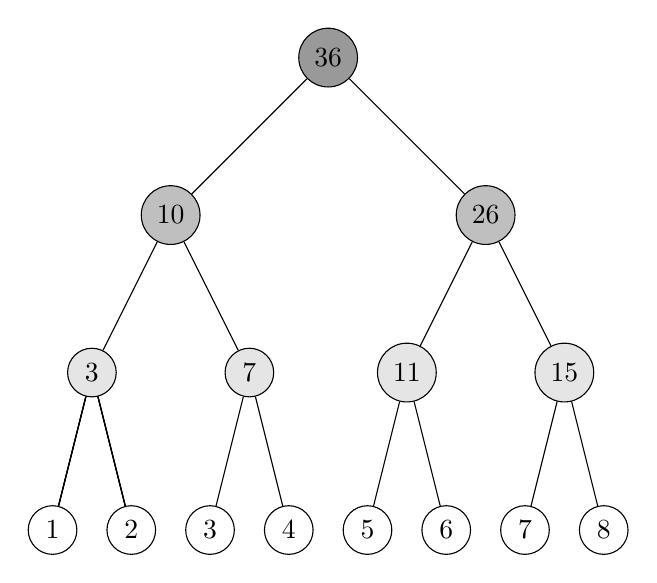
\begin{tikzpicture}
            \node[draw,circle] (A1) at (1, 0) { 1 };
            \node[draw,circle] (A2) at (2, 0) { 2 };
            \node[draw,circle] (A3) at (3, 0) { 3 };
            \node[draw,circle] (A4) at (4, 0) { 4 };
            \node[draw,circle] (A5) at (5, 0) { 5 };
            \node[draw,circle] (A6) at (6, 0) { 6 };
            \node[draw,circle] (A7) at (7, 0) { 7 };
            \node[draw,circle] (A8) at (8, 0) { 8 };

            \node[draw,circle,fill=gray!20] (B1) at (1.5, 2) { 3 };
            \node[draw,circle,fill=gray!20] (B2) at (3.5, 2) { 7 };
            \node[draw,circle,fill=gray!20] (B3) at (5.5, 2) { 11 };
            \node[draw,circle,fill=gray!20] (B4) at (7.5, 2) { 15 };

            \node[draw,circle,fill=gray!50] (C1) at (2.5, 4) { 10 };
            \node[draw,circle,fill=gray!50] (C2) at (6.5, 4) { 26 };

            \node[draw,circle,fill=gray!80] (D1) at (4.5, 6) { 36 };

            \draw (A1) -- (B1);
            \draw (A2) -- (B1);
            \draw (A3) -- (B2);
            \draw (A4) -- (B2);
            \draw (A5) -- (B3);
            \draw (A6) -- (B3);
            \draw (A7) -- (B4);
            \draw (A8) -- (B4);
            \draw (A1) -- (B1);
            \draw (A2) -- (B1);
            \draw (A1) -- (B1);
            \draw (A2) -- (B1);
            \draw (A1) -- (B1);
            \draw (A2) -- (B1);
            \draw (B1) -- (C1);
            \draw (B2) -- (C1);
            \draw (B3) -- (C2);
            \draw (B4) -- (C2);
            \draw (C1) -- (D1);
            \draw (C2) -- (D1);
        \end{tikzpicture}
    \end{figure}

\end{frame}
